\documentclass[tikz,border=3pt]{standalone}
\usepackage[utf8]{inputenc}
\usepackage[T1]{fontenc}
\usepackage{lmodern}
\renewcommand{\familydefault}{\sfdefault}
\usepackage{sansmath}\sansmath
\usepackage{chemfig}
\usepackage{pgfplots}\pgfplotsset{compat=1.18,/pgf/number format/use comma,/pgf/number format/1000 sep={.}}
\usetikzlibrary{arrows.meta,calc,positioning,decorations.pathmorphing,patterns}
% paleta del sitio
\definecolor{nar}{HTML}{E8680C}\definecolor{narc}{HTML}{FFB35C}\definecolor{hielo}{HTML}{FFF3E8}
\definecolor{tinta}{HTML}{1D1D1F}\definecolor{gris}{HTML}{6E6E73}\definecolor{lila}{HTML}{7C5CF0}
\definecolor{azul}{HTML}{2F6FD6}\definecolor{menta}{HTML}{17A673}\definecolor{coral}{HTML}{E8342A}
\tikzset{cel/.style={draw=gris,fill=hielo,line width=0.9pt},nuc/.style={draw=gris!70,line width=0.6pt},
fib/.style={gris!55,line width=0.35pt},eti/.style={font=\footnotesize,text=tinta,align=center},
num/.style={circle,draw=nar,fill=white,text=nar,font=\small\bfseries,inner sep=1.2pt,minimum size=13pt},
fl/.style={-{Stealth[length=2.6mm]},gris,line width=0.9pt}}
\begin{document}
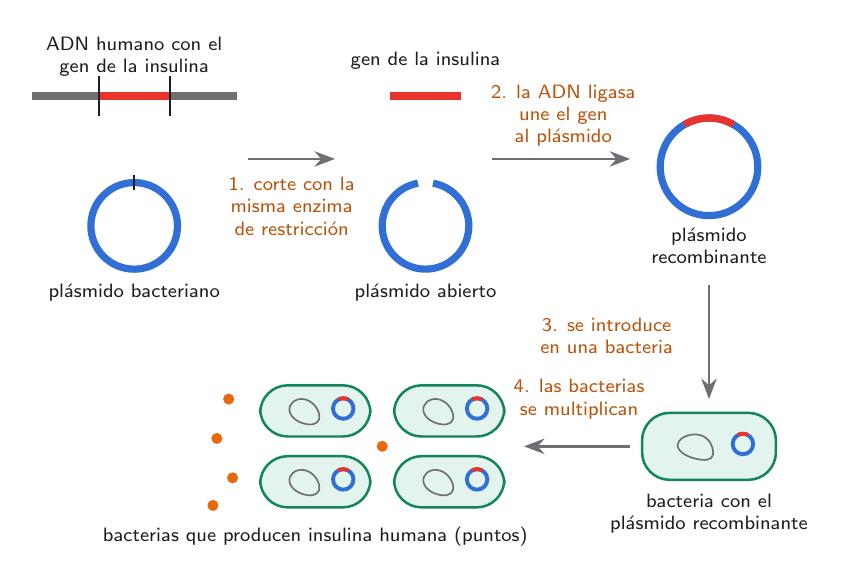
\begin{tikzpicture}[font=\small]
\draw[gris,line width=3pt] (0,1.0)--(2.6,1.0);\draw[coral,line width=3pt] (0.85,1.0)--(1.75,1.0);
\draw[tinta,thick] (0.85,0.75)--(0.85,1.25) (1.75,0.75)--(1.75,1.25);
\node[eti,font=\scriptsize] at (1.3,1.5) {ADN humano con el\\gen de la insulina};
\draw[azul,line width=2.6pt] (1.3,-0.65) circle (0.55);
\draw[tinta,thick] (1.3,-0.2)--(1.3,0.0);
\node[eti,font=\scriptsize] at (1.3,-1.5) {plásmido bacteriano};
\draw[coral,line width=3pt] (4.55,1.0)--(5.45,1.0);
\node[eti,font=\scriptsize] at (5,1.45) {gen de la insulina};
\draw[azul,line width=2.6pt] (4.904,-0.108) arc (100:440:0.55);
\node[eti,font=\scriptsize] at (5,-1.5) {plásmido abierto};
\draw[azul,line width=2.6pt] (8.6,0.1) circle (0.62);
\draw[coral,line width=2.6pt] (8.91,0.637) arc (60:120:0.62);
\node[eti,font=\scriptsize] at (8.6,-0.9) {plásmido\\recombinante};
\draw[menta!80!black,fill=menta!12,line width=0.9pt,rounded corners=3.5mm] (7.75,-3.875) rectangle (9.45,-3.025);
\draw[gris,line width=0.6pt] plot[smooth cycle,tension=1] coordinates {(8.203,-3.45) (8.45,-3.3) (8.65,-3.5) (8.5,-3.62)};
\draw[azul,line width=1.4pt] (9.031,-3.42) circle (0.13);
\draw[coral,line width=1.4pt] (9.096,-3.307) arc (60:120:0.13);
\node[eti,font=\scriptsize] at (8.6,-4.3) {bacteria con el\\plásmido recombinante};
\draw[menta!80!black,fill=menta!12,line width=0.9pt,rounded corners=3.5mm] (4.6,-3.325) rectangle (6,-2.675);
\draw[gris,line width=0.6pt] plot[smooth cycle,tension=1] coordinates {(4.973,-3) (5.15,-2.85) (5.35,-3.05) (5.2,-3.17)};
\draw[azul,line width=1.4pt] (5.655,-2.97) circle (0.13);
\draw[coral,line width=1.4pt] (5.72,-2.857) arc (60:120:0.13);
\draw[menta!80!black,fill=menta!12,line width=0.9pt,rounded corners=3.5mm] (2.9,-3.325) rectangle (4.3,-2.675);
\draw[gris,line width=0.6pt] plot[smooth cycle,tension=1] coordinates {(3.273,-3) (3.45,-2.85) (3.65,-3.05) (3.5,-3.17)};
\draw[azul,line width=1.4pt] (3.955,-2.97) circle (0.13);
\draw[coral,line width=1.4pt] (4.02,-2.857) arc (60:120:0.13);
\draw[menta!80!black,fill=menta!12,line width=0.9pt,rounded corners=3.5mm] (4.6,-4.225) rectangle (6,-3.575);
\draw[gris,line width=0.6pt] plot[smooth cycle,tension=1] coordinates {(4.973,-3.9) (5.15,-3.75) (5.35,-3.95) (5.2,-4.07)};
\draw[azul,line width=1.4pt] (5.655,-3.87) circle (0.13);
\draw[coral,line width=1.4pt] (5.72,-3.757) arc (60:120:0.13);
\draw[menta!80!black,fill=menta!12,line width=0.9pt,rounded corners=3.5mm] (2.9,-4.225) rectangle (4.3,-3.575);
\draw[gris,line width=0.6pt] plot[smooth cycle,tension=1] coordinates {(3.273,-3.9) (3.45,-3.75) (3.65,-3.95) (3.5,-4.07)};
\draw[azul,line width=1.4pt] (3.955,-3.87) circle (0.13);
\draw[coral,line width=1.4pt] (4.02,-3.757) arc (60:120:0.13);
\fill[nar] (2.5,-2.85) circle (2pt);
\fill[nar] (2.35,-3.35) circle (2pt);
\fill[nar] (2.55,-3.85) circle (2pt);
\fill[nar] (2.3,-4.2) circle (2pt);
\fill[nar] (4.45,-3.45) circle (2pt);
\node[eti,font=\scriptsize] at (3.6,-4.6) {bacterias que producen insulina humana (puntos)};
\draw[fl] (2.75,0.2)--(3.85,0.2);
\node[font=\scriptsize,text=nar!80!black,align=center] at (3.3,-0.4) {1. corte con la\\misma enzima\\de restricción};
\draw[fl] (5.85,0.2)--(7.6,0.2);
\node[font=\scriptsize,text=nar!80!black,align=center] at (6.75,0.75) {2. la ADN ligasa\\une el gen\\al plásmido};
\draw[fl] (8.6,-1.4)--(8.6,-2.85);
\node[font=\scriptsize,text=nar!80!black,align=center] at (7.3,-2.05) {3. se introduce\\en una bacteria};
\draw[fl] (7.6,-3.45)--(6.25,-3.45);
\node[font=\scriptsize,text=nar!80!black,align=center] at (6.95,-2.85) {4. las bacterias\\se multiplican};
\end{tikzpicture}
\end{document}
